\documentclass{beamer}

%\documentclass[12pt,xcolor=dvipsname,handout]{beamer}
\setbeamertemplate{navigation symbols}{}

\setbeamercolor{frametitle}{fg=black,bg=white}
\setbeamercolor{title}{fg=black,bg=yellow!85!orange}
\usetheme{AnnArbor}

\usepackage{graphicx} % Allows including images
\usepackage{booktabs} % Allows the use of \toprule, \midrule and \bottomrule in tables

\beamersetuncovermixins{\opaqueness<1>{25}}{\opaqueness<2->{15}}
\begin{document}
\title[q-PCR accuracy]{An assessment of q-PCR accuracy based on RNA-seq} % The short title appears at the bottom of every slide, the full title is only on the title page

\author[V. Sherina]{presented by V. Sherina} % Your name
%\institute[UR] % Your institution as it will appear on the bottom of every slide, may be shorthand to save space
%{
%Georgia Southern University \\ % Your institution for the title page
%\medskip
%\textit{vs00769@georgiasouthern.edu} % Your email address
%}
\date{October 7, 2015} % Date, can be changed to a custom date
\begin{frame}
\titlepage
\end{frame}
%---------------------------------------------------------
%\begin{frame}\frametitle{Table of contents}
%\begin{small}
%\tableofcontents
%\end{small}
%\end{frame} 
%---------------------------------------------------------
\section{Introduction}
\begin{frame}
\frametitle{Introduction}
  \begin{columns}[T]
    \begin{column}{.6\textwidth}
     \begin{block}{}
% Your text here
The {\bf National Center for Biotechnology Information} (NCBI) is part of the United States National Library of Medicine (NLM), a branch of the National Institutes of Health.  \pause\\ 
\hspace{0.3cm} \\
The NCBI is located in Maryland and was founded in 1988 through legislation sponsored by Senator Claude Pepper.
    \end{block}
    \end{column}
    \begin{column}{.4\textwidth}
    \begin{block}{}
% Your image included here
    
\includegraphics[width=0.9\textwidth]{table1.png}
    \end{block}
    \end{column}
  \end{columns}
\end{frame}
%---------------------------------------------------------

\begin{frame}
\frametitle{Introduction}
The NCBI houses 
\begin{itemize}
\item a series of databases biotechnology and biomedicine;\pause
\item and an important resource for bioinformatics tools and services. \pause
\end{itemize}
\vspace{0.3cm}
Major databases 
\begin{itemize}
\item {\bf GenBank} for DNA sequences, \pause
\item {\bf PubMed}, a bibliographic database for the biomedical literature, \pause
\item the {\bf NCBI Epigenomics} database, \pause
\item {\bf Gene Expression Omnibus} (GEO).\pause
\end{itemize}
All these databases are available online through the {\bf Entrez} search engine.
\end{frame}
%---------------------------------------------------------

\begin{frame}
\frametitle{GEO}
{\bf GEO} is a public functional genomics data repository supporting MIAME-compliant data submissions. Array- and sequence-based data are accepted.\par Tools are provided to help users query and download experiments and curated gene expression profiles.

\end{frame}
%---------------------------------------------------------
\section{Motivation}
\begin{frame}
\frametitle{Motivation}
\begin{itemize}
\item "A comprehensive assessment of RNA-seq accuracy, reproducibility and information content by the sequencing quality control consortium." Nature Biotechnology (2014), by SEQC/MAQC-III Consortium.
\pause
\item Bioconductor package with data "RNA-seq data generated from SEQC (MAQC-III) study", by Yang Liao and Wei Shi with contributions from Steve Lianoglou.
\pause
\end{itemize}
\end{frame}
%---------------------------------------------------------

\begin{frame}
\frametitle{Results}
The Sequencing Quality Control (SEQC) project is coordinated by the US FDA. 
Examining Illumina HiSeq, Life Technologies SOLiD and Roche 454 platforms at multiple laboratory sites using reference RNA samples with built-in controls, authors
\begin{itemize}
\item Assess RNA sequencing (RNA-seq) performance for junction discovery and differential expression profiling.\pause 
\item Using complementary metrics, compare it to microarray data, \pause
\item and compare it to quantitative PCR (q-PCR) data.
\end{itemize} 
\end{frame}
%---------------------------------------------------------

\begin{frame}
\frametitle{Cross-platform agreement of expression levels}

(a) Comparison of log2 fold-change estimates for 843 selected genes. Good and similar concordances were observed between relative expression measures from the MAQC-III HiSeq 2000 and SOLiD sequencing platforms, MAQC-I TaqMan and the MAQC-III Affymetrix HuGene2 arrays (Pearson and Spearman correlation)
\vspace{0.3cm}
(d) Comparison of TaqMan and PrimePCR for 843 selected genes.
\end{frame}
%---------------------------------------------------------

\begin{frame}
%\frametitle{SMART example}
\begin{figure}[h!]
\centerline{
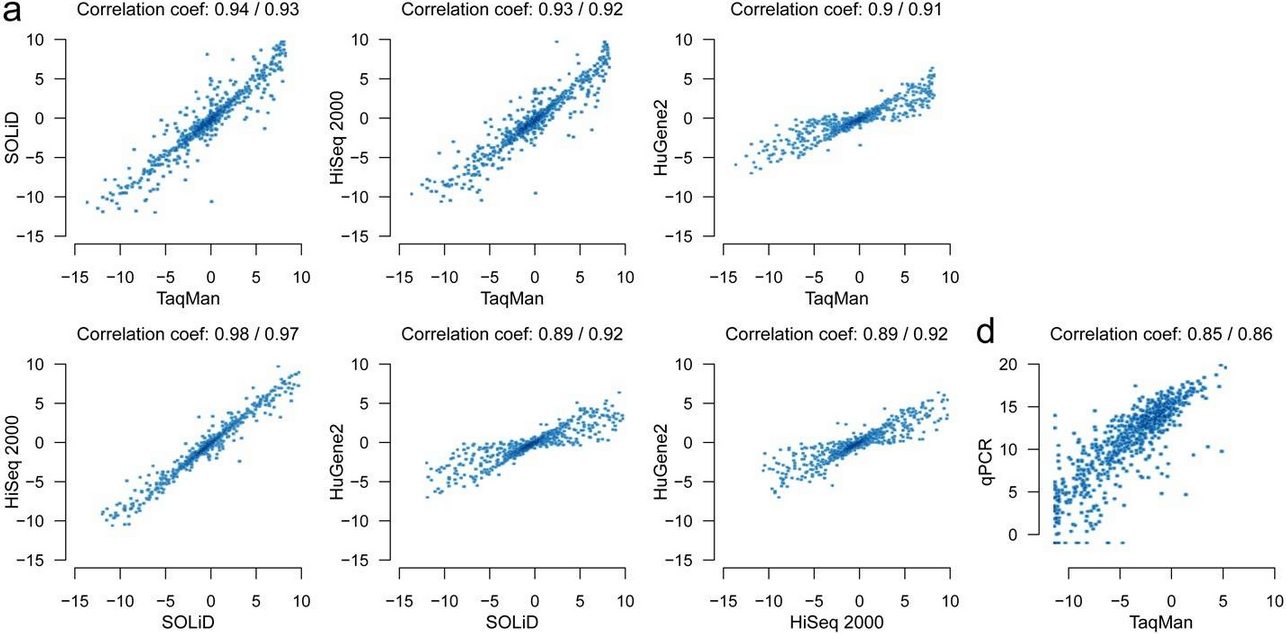
\includegraphics[width=0.9\textwidth]{table2.png}}
\label{fig:1}       
\end{figure}
\pause Expression estimates vary considerably for individual genes, with some genes showing high expression in one platform but are not detected at all by the other.
\end{frame}
%---------------------------------------------------------

\begin{frame}
\frametitle{"Gold" standard}
{\bf q-PCR-based methods}:
\begin{itemize}
\item high sensitivity; \pause
\item and dynamic range. \pause
\item q-PCR traditionally been used as a reference "gold" standard. \pause
\end{itemize} 
\vspace{0.3cm}
\begin{itemize}
\item One challenge of q-PCR data is the presence of non-detects (those reactions failing to attain the expression threshold).\pause
\item While most current software replaces these non-detects with  the  maximum  possible  Ct  value,  recent  work  has  shown  that this introduces large biases in estimation of both absolute and differential expression.\cite{McCall} \pause
\item Considerable differences in expression level measurements from different PCR-based assays can be observed.
\end{itemize}
\end{frame}

%---------------------------------------------------------

\section{Project Proposal}
\begin{frame}
\frametitle{Ideas}
\begin{itemize}
\item Validation has been an important part in RNA-seq publication. The differentially expressed genes (at least some) identified using RNA-seq are often validated using q-PCR. \pause
\item I am going to identify specific genes, where results of RNA-seq and q-PCR disagree.\pause
\item If the disagreement caused by low detection in q-PCR experiment, it may be possible to estimate non-detected Ct values, and  repeat the validation procedure. \pause
\item The claim of the project is q-PCR results may be validated using RNA-seq data. 
\end{itemize}  
\end{frame}
%---------------------------------------------------------

\begin{frame}
\frametitle{References}
\begin{footnotesize}
\begin{thebibliography}{X}

\bibitem{SEQC} 
SEQC/MAQC-III Consortium \textit {A comprehensive assessment of RNA-seq accuracy, reproducibility and information content by the Sequencing Quality Control Consortium} Nature Biotechnology 32, 903–914, 2014.

\bibitem{McCall}
M.N. McCall, H.R. McMurray, H. Land and A. Almudevar \textit {On non-detects in Quantitative real-time PCR data.} Bioinformatics V. 30 no. 16, 2310-2316, 2014.
%%
%%\bibitem{B60}
%%Bjerkedal, T., \emph{Acquisition of resistance in guinea pigs infected with different doses of virulent tubercle bacilli}, American Journal of Hygiene, vol. 72, 130-148 (1960).
%%%
%%\bibitem{C89}
%%Calabria, R., Pulcini, G., \emph{Confidence limits for reliability and tolerance limits in the inverse Weibull distribution}, Engineering and System Safety, 24, 77-85 (1989).
%%
%%\bibitem{C90}
%%Calabria, R., Pulcini, G., \emph{On the maximum likelihood and least squares estimation in inverse Weibull distribution,} Statistica Applicata, 2, 53-66 (1990). 
%%
%%\bibitem {C94}
%%Calabria, R., Pulcini, G., \emph{Bayes 2-sample prediction for the inverse Weibull distribution,} Communications in Statistics-Theory Meth., 23(6), 1811-1824 (1994).
%%
\end{thebibliography}
\end{footnotesize}
\end{frame}
%----------------------------------------------------------

\begin{frame}
\begin{center}
\begin{Huge}
Thank you for your attention! \pause\\ Questions?
\end{Huge}
\end{center}
\end{frame}

%----------------------------------------------------------

\end{document}
